\documentclass[11pt,a4paper]{article}

\usepackage[utf8]{inputenc}
\usepackage[T1]{fontenc}
\usepackage{lmodern}
\usepackage[ngerman]{babel}
\usepackage{amsmath,amssymb,amsthm,mathtools}
\usepackage{booktabs}
\usepackage{microtype}
\usepackage{graphicx}
\usepackage{xcolor}
\usepackage{geometry}
\geometry{a4paper, left=25mm, right=25mm, top=25mm, bottom=25mm}
\usepackage{hyperref}
\hypersetup{
    colorlinks=true,
    linkcolor=blue!80!black,
    citecolor=blue!80!black,
    urlcolor=blue!80!black
}

\theoremstyle{plain}
\newtheorem{theorem}{Satz}[section]
\newtheorem{lemma}[theorem]{Lemma}
\newtheorem{corollary}[theorem]{Korollar}
\newtheorem{proposition}[theorem]{Proposition}

\theoremstyle{definition}
\newtheorem{definition}[theorem]{Definition}
\newtheorem{remark}[theorem]{Bemerkung}

\newcommand{\N}{\mathbb{N}}
\newcommand{\Z}{\mathbb{Z}}
\newcommand{\Q}{\mathbb{Q}}
\newcommand{\R}{\mathbb{R}}
\newcommand{\OK}{\mathcal{O}_K}
\newcommand{\E}{\mathbb{E}}
\DeclareMathOperator{\rank}{rank}
\DeclareMathOperator{\diag}{diag}
\DeclareMathOperator{\Tr}{Tr}
\numberwithin{equation}{section}

\title{\textbf{Historische und mathematische Einordnung\\
der Phasenraumtransformation $\Psi_{9,\log}^{(2)}$}}
\author{\textbf{Thomas Hoffbauer}\\ Bamberg}
\date{Oktober 2026}

\begin{document}
\maketitle

\begin{abstract}
\noindent
Dieser Bericht ordnet die geometrische Phasenraumtransformation
$\Psi_{9,\log}^{(2)}$ in die beiden Traditionen ein, aus denen sie gebaut ist:
die Collatz--Syracuse-Dynamik seit 1937 und die Minkowski-Einbettung des
reell-quadratischen Körpers $\Q(\sqrt{5})$.
Die Note, die hier gelesen wird, beweist drei strukturelle Sätze.
Der reelle Spann der Bildmenge hat die Dimension~$9$.
Die beschleunigte ungerade Abbildung
$T_*(o)=(3o+1)/2^{v_2(3o+1)}$ landet nach einem Schritt auf der
linearen Hyperfläche $H=\{\tau-2(U_0+S_0)=0\}$.
Der orthogonale Projektor auf $H$ zerlegt $\R^9$ kanonisch als
$\R^3_U\oplus\R^2_B\oplus\R^3_S\oplus\R_N$.

Dieselben Sätze werden hier an ihre klassischen Quellen gebunden.
Die transverse Koordinate $\delta_{\mathrm{can}}$ ist der Fundamentbereich des
Dirichletschen Regulatorgitters von $\Q(\sqrt{5})$, gefaltet unter der
Galois-Konjugation.
Die vier EABC-Klassen sind die Charaktergruppe von $(\Z/12\Z)^\times$.
Der negative Skalendrift $\log(3/4)$ ist der Erwartungswert eines
beschleunigten Schritts unter dem Haar-Maß auf $\Z_2^\times$;
der in der Übersichtsliteratur übliche Wert $\tfrac12\log(3/4)$ ist derselbe
Zufallsgang, gezählt in Einzelschritten der Abbildung von Lagarias.
Eine Stichprobe von $100\,000$ Schritten bestätigt das geometrische Gesetz
$\Pr(v_2(3o+1)=k)=2^{-k}$ und liefert den empirischen Mittelwert
$-0{,}290233$ gegen $\log(3/4)\approx -0{,}287682$.
Die Differenz liegt innerhalb einer Standardabweichung des Stichprobenmittels.

Die Collatz-Vermutung bleibt offen.
Der Bericht trennt, was die Konstruktion beweist, was sie aus der klassischen
Theorie übernimmt, und welche Aussage über einzelne Bahnen weiterhin eine
Modellannahme über den Faktorisierungsdefekt $D_3$ ist.
\end{abstract}

\noindent\textbf{MSC (2020):} 11B83, 11R11, 11S82, 37A45.\\
\textbf{Schlüsselwörter:} Collatz-Vermutung, Syracuse-Abbildung, Haar-Maß auf $\Z_2^\times$,
Minkowski-Einbettung, $\Q(\sqrt{5})$, Walsh-Analyse modulo~$12$.

\tableofcontents
\newpage

%==============================================================================
\section{Gegenstand und Geltungsbereich}
%==============================================================================

Ausgangspunkt ist die Note über die Transformation $\Psi_{9,\log}^{(2)}$ und die
Hyperfläche~$H$ \cite{Psi9}.
Sie führt auf $\N_{>0}$ einen Vektor in $\R^9$ ein, dessen erste Koordinate der
archimedische Logarithmus $\tau(n)=\log n$ ist und dessen übrige acht Koordinaten
aus einer logarithmischen Einbettung der Primfaktoren $p>3$ entstehen.
Die Einbettung benutzt den Ganzheitsring $\Z[\phi]$ des Körpers $\Q(\sqrt{5})$
und anschließend die Walsh--Hadamard-Matrix der Ordnung~$4$.

Der vorliegende Text wiederholt die Definitionen und die drei Hauptbeweise so,
dass jede Konstruktion an der Stelle steht, an der sie historisch und
algebraisch hingehört.
Vier Leitfragen ordnen das Material.

\begin{enumerate}
\item Welches Stück der Konstruktion ist Collatz-Dynamik, welches Stück ist
algebraische Zahlentheorie, und welches Stück ist Fourier-Analyse auf einer
endlichen abelschen Gruppe?
\item Warum liefert gerade die Zerlegung von Primzahlen in $\Q(\sqrt{5})$ den
vollen Rang~$9$, während träge Primzahlen allein ihn nicht ergeben?
\item In welcher Normierung ist der theoretische Drift $\log(3/4)$, und wie
verhält er sich zu der Steigung $\tfrac12\log(3/4)$, die seit Terras und
Lagarias für die Einzelschritt-Abbildung angegeben wird?
\item Welche der Aussagen gelten für jede einzelne Bahn, und welche gelten als
Erwartungswert unter dem Haar-Maß?
\end{enumerate}

Die Antwort auf die vierte Frage bestimmt den Geltungsbereich.
Rang, Kollaps auf $H$ und die Hauptachsenzerlegung sind Sätze über die
Einbettung und über einen einzelnen beschleunigten Schritt.
Der negative Erwartungswert des Skaleninkrements ist ein Satz über das
Haar-Maß auf den $2$-adischen Einheiten.
Eine gleichmäßige Schranke, die jede Startzahl nach endlich vielen Schritten
unter eine feste Höhe drückt, liegt außerhalb dieses Rahmens.
In dieser Hinsicht schließt der Bericht an die frühere Trennung von Bestand,
Sonde und offener Lücke an \cite{CollatzE8}.

%==============================================================================
\section{Die Collatz-Abbildung in der historischen Literatur}
%==============================================================================

\subsection{Entstehung und äquivalente Formulierungen}

Lothar Collatz hat die Iteration, die heute seinen Namen trägt, nach eigener
späterer Auskunft im Jahr 1937 untersucht und zunächst nicht veröffentlicht.
Sie zirkulierte unter mehreren Namen: als Syracuse-Problem in der Umgebung von
Helmut Hasse, als Problem von Kakutani und als Problem von Ulam.
Die maßgebliche mathematische Kodifikation ist der Überblick von Lagarias
\cite{Lagarias1985}, fortgeschrieben in der Sammelmonographie von 2010 und in
der aktualisierten Übersicht \cite{Lagarias2021}.

Zwei Normalisierungen derselben Bahn werden nebeneinander gebraucht.
Die unkomprimierte Abbildung sendet ein ungerades $n$ auf $3n+1$ und ein
gerades $n$ auf $n/2$.
Ihr attraktiver Zyklus, falls die Vermutung zutrifft, ist $\{1,4,2\}$.
Die in der analytischen Literatur übliche Abbildung von Lagarias fasst den
ungeraden Schritt bereits mit einer Zweierdivision zusammen,
\begin{equation}
\label{eq:Tlagarias}
T(n)=
\begin{cases}
n/2, & n\equiv 0\pmod{2},\\[0.3em]
(3n+1)/2, & n\equiv 1\pmod{2}.
\end{cases}
\end{equation}
Die Note und dieser Bericht arbeiten mit der noch stärker beschleunigten
ungeraden Abbildung
\begin{equation}
\label{eq:Tstar}
T_*:\N_{\mathrm{odd}}\to\N_{\mathrm{odd}},
\qquad
T_*(o)=\frac{3o+1}{2^{k(o)}},
\qquad
k(o)=v_2(3o+1).
\end{equation}
Ein Schritt von $T_*$ ist genau ein Übergang von einer ungeraden Zahl zur
nächsten ungeraden Zahl.
Die drei Beschreibungen erzeugen dieselben ungeraden Terme einer Bahn.
Sie unterscheiden sich in der Zählung der Schritte und deshalb im numerischen
Wert des mittleren logarithmischen Drifts.
Abschnitt~\ref{sec:drift} rechnet diese Beziehung explizit um.

Die Vermutung besagt, dass jede positive ganze Zahl den Zyklus durch~$1$
erreicht.
Sie ist offen.
Veröffentlicht sind drei Arten von Teilresultaten, die den Rahmen für jede
geometrische Uminterpretation abgeben.

\begin{enumerate}
\item \textbf{Verifikation bis zu einer expliziten Schranke.}
Barina hat die Konvergenz aller Startwerte unterhalb von $2^{71}$ nachgewiesen
\cite{Barina2025}; die Schwelle $2^{68}$ war der Stand von 2020 \cite{Barina2021}.
\item \textbf{Dichtesätze.}
Korec zeigte, dass für jedes $\theta>\log 3/\log 4$ fast alle Startwerte,
im Sinn der natürlichen Dichte, in ihrer Bahn unter $n^{\theta}$ fallen
\cite{Korec1994}.
Tao verschärfte dies zur logarithmischen Dichte: für jede Funktion
$f(N)\to\infty$ gilt $\mathrm{Col}_{\min}(N)<f(N)$ für fast alle $N$
\cite{Tao2019}.
\item \textbf{Zyklen endlicher Länge.}
Steiner schloss nichttriviale $1$-Zyklen aus \cite{Steiner1977}.
Simons und de Weger gaben Schranken für $m$-Zyklen mit kleinem $m$
\cite{SimonsDeWeger2005}.
Ein Ausschluss beliebiger Perioden fehlt.
\end{enumerate}

Zwei Hindernisse bleiben damit in der klassischen Form bestehen: eine
unbeschränkte Bahn und ein fremder Zyklus \cite{Lagarias1985,CollatzE8}.

\subsection{Warum die Koeffizienten 3 und 2 speziell sind}

Conway bewies 1972, dass eine naheliegende Verallgemeinerung, in der die
affinen Zweige $an+b$ von der Restklasse modulo einer festen Zahl abhängen,
im Allgemeinen algorithmisch unentscheidbar ist \cite{Conway1972}.
Ein Beweis für die konkrete Abbildung muss deshalb die besonderen Koeffizienten
$3$ und $2$ benutzen.
In logarithmischer Gestalt ist die einzige aus diesen Koeffizienten gebildete
Kontraktionsgröße das Verhältnis $\log 3/\log 2$, beziehungsweise die
Differenz $\log 3-2\log 2=\log(3/4)<0$, sobald ein ungerader Schritt im Mittel
zwei Zweierdivisionen nach sich zieht.
Jede geometrische Verpackung der Dynamik, die einen negativen Drift ausweist,
rechnet an dieser Stelle mit derselben klassischen Größe.
Sie entsteht nicht aus der Wahl des Hilfskörpers $\Q(\sqrt{5})$.

\subsection{Das 2-adische Modell von Terras und Everett}

Terras \cite{Terras1976} und Everett \cite{Everett1977} beobachteten, dass die
ersten Paritäten einer Bahn sich wie unabhängige Münzwürfe verhalten, solange
man nur Kongruenzbedingungen modulo einer festen Zweierpotenz stellt.
Daraus wurde das Restklassenmodell, das Lagarias als Standardheuristik
formuliert hat \cite{Lagarias1985,Lagarias2021}: entlang einer typischen Bahn
ist der logarithmische Graph näherungsweise eine Gerade mit negativer Steigung.

Für die Einzelschritt-Abbildung~\eqref{eq:Tlagarias} lautet diese Steigung
\begin{equation}
\label{eq:steigungT}
-\frac12\log\frac34 \approx -0{,}143841.
\end{equation}
Die zugehörige mittlere Schrittzahl bis zur Höhe~$1$ ist
$2\log n\big/\log(4/3)\approx 6{,}952\,\log n$.
Abschnitt~\ref{sec:drift} zeigt, dass~\eqref{eq:steigungT} und der Drift
$\log(3/4)$ der beschleunigten Abbildung~\eqref{eq:Tstar} dieselbe
Zufallsgröße in zwei Zählungen sind.
Die numerische Figur am Ende dieses Berichts prüft die beschleunigte Zählung.

%==============================================================================
\section{Der Körper \texorpdfstring{$\Q(\sqrt{5})$}{Q(sqrt(5))}
und seine Minkowski-Einbettung}
%==============================================================================

\subsection{Ganzheitsring, Verzweigung und Klassenzahl}

Sei $K=\Q(\sqrt{5})$.
Die Diskriminante ist $D_K=5$.
Da $5\equiv 1\pmod{4}$ gilt, ist der Ganzheitsring gegeben durch
\begin{equation}
\OK=\Z\!\left[\frac{1+\sqrt{5}}{2}\right]=\Z[\phi],
\qquad
\phi=\frac{1+\sqrt{5}}{2}.
\end{equation}
Die beiden reellen Einbettungen $\sigma_+,\sigma_-:K\to\R$ sind durch
$\sqrt{5}\mapsto\pm\sqrt{5}$ bestimmt.
Insbesondere ist $\sigma_+(\phi)=\phi$ und $\sigma_-(\phi)=\phi'=(1-\sqrt{5})/2=-1/\phi$,
also $\lvert\phi'\rvert=\phi^{-1}$.
Die Norm $N(\alpha)=\sigma_+(\alpha)\sigma_-(\alpha)$ ist auf $\OK$ die binäre Form
\begin{equation}
\label{eq:normform}
N(a+b\phi)=a^2+ab-b^2,\qquad a,b\in\Z.
\end{equation}
Sie ist die Hauptform der Diskriminante~$5$.
Ihre Darstellungstheorie gehört zum ältesten Bestand der quadratischen Formen,
von der Theorie des regelmäßigen Fünfecks bis zu Gauss.

\begin{proposition}[Zerlegungsgesetz]
Für eine ungerade Primzahl $p\neq 5$ gilt:
\begin{enumerate}
\item $p\equiv \pm 1\pmod{5}$, das heißt $p\equiv 1,4\pmod{5}$:
$(p)=\mathfrak{p}\,\overline{\mathfrak{p}}$ zerfällt in zwei verschiedene Primideale der Norm~$p$.
\item $p\equiv \pm 2\pmod{5}$, das heißt $p\equiv 2,3\pmod{5}$:
$(p)$ bleibt träge.
\end{enumerate}
Die Primzahl $5$ ist verzweigt, $(5)=(\sqrt{5})^2$ bis auf Einheiten.
Die Primzahlen $2$ und $3$ sind träge.
\end{proposition}

\begin{proof}
Das Legendre-Symbol $\bigl(\frac{5}{p}\bigr)$ entscheidet nach dem
Kummerschen Zerlegungsgesetz über das Verhalten von~$p$.
Da $5\equiv 1\pmod{4}$, liefert das quadratische Reziprozitätsgesetz
$\bigl(\frac{5}{p}\bigr)=\bigl(\frac{p}{5}\bigr)$.
Die quadratischen Reste modulo~$5$ sind $0,1,4$.
Also ist $\bigl(\frac{p}{5}\bigr)=1$ genau für $p\equiv 1,4\pmod{5}$.
Die Diskriminante wird nur von~$5$ geteilt, daher ist $5$ die einzige
verzweigte Primzahl.
Modulo~$8$ ist $5\equiv 5\pmod{8}$, also bleibt $2$ träge.
Wegen $\bigl(\frac{3}{5}\bigr)=-1$ bleibt auch $3$ träge.
\end{proof}

Die beiden Collatz-Koeffizienten $2$ und $3$ liegen damit außerhalb der
Menge der zerlegten Primzahlen.
In der Transformation werden sie ohnehin aus dem internen Faktorisierungsvektor
herausgezogen und nur in der Normalenkoordinate von~$H$ geführt.
Der Körper $\Q(\sqrt{5})$ ist dafür nicht logisch erzwungen.
Er ist der reell-quadratische Körper kleinster Diskriminante, mit
Klassenzahl eins und kleinstem Regulator.
Dieselbe Rangrechnung ließe sich in jedem anderen reell-quadratischen
Hauptidealring mit einer analogen Querkoordinate wiederholen.
Die Dynamik von $T_*$ hängt an $2$ und $3$; der Körper liefert das
Koordinatensystem.

\begin{proposition}[Klassenzahl]
Die Klassenzahl von $K=\Q(\sqrt{5})$ ist $h_K=1$.
Jedes gebrochene Ideal ist ein Hauptideal, und jede zerlegte rationale
Primzahl $q$ besitzt einen Erzeuger $\pi\in\OK$ mit $\lvert N(\pi)\rvert=q$.
\end{proposition}

\begin{proof}
Die Minkowski-Schranke eines Zahlkörpers vom Grad $n$ mit $r_2$ Paaren
komplexer Einbettungen und Diskriminante $D$ lautet
\begin{equation}
M_K=\frac{n!}{n^n}\Bigl(\frac{4}{\pi}\Bigr)^{r_2}\sqrt{\lvert D\rvert}.
\end{equation}
Hier ist $n=2$, $r_2=0$ und $D=5$, also
$M_K=\frac12\sqrt{5}\approx 1{,}118<2$.
Jede Idealklasse enthält ein ganzes Ideal der Norm höchstens $M_K$,
mithin der Norm~$1$.
Das einzige solche Ideal ist $(1)$.
Folglich ist $h_K=1$.
Ein zerlegtes Primideal der Norm~$q$ ist daher ein Hauptideal $(\pi)$ mit
$\lvert N(\pi)\rvert=q$.
\end{proof}

Ohne Klassenzahl eins wäre ein zerlegtes Primideal im Allgemeinen kein
Hauptideal, und die in der Note verwendete Erzeugerwahl $\pi\in\OK$ wäre nur
für Hauptprimideale erklärt.
Für $\Q(\sqrt{5})$ ist diese Einschränkung leer.
Für den Rang-Satz weiter unten genügen zudem vier explizite Erzeuger;
dieser Satz benutzt die allgemeine Klassenzahl nicht.

\subsection{Dirichletscher Einheitensatz und der Regulator}

Nach dem Einheitensatz von Dirichlet hat die Einheitengruppe eines
reell-quadratischen Körpers den Rang $r_1+r_2-1=1$.
Eine Fundamentaleinheit von $\OK$ ist $\phi$ selbst, mit Norm
\begin{equation}
N(\phi)=\phi\cdot\phi'=-1.
\end{equation}
Die volle Einheitengruppe ist $\{\pm\phi^k:k\in\Z\}$.
Die logarithmische Einbettung
\begin{equation}
\lambda:\OK^\times\to\R^2,
\qquad
\lambda(\varepsilon)=\bigl(\log\lvert\sigma_+(\varepsilon)\rvert,\,
\log\lvert\sigma_-(\varepsilon)\rvert\bigr)
\end{equation}
landet in der Spur-Null-Geraden $x+y=0$, weil $\lvert N(\varepsilon)\rvert=1$.
Das Bild von $\langle\phi\rangle$ ist das Gitter $\Z\cdot(\log\phi,-\log\phi)$.
Der Regulator, also der Covolumen-Faktor dieses Gitters in der Geraden, ist
\begin{equation}
R_K=\log\phi\approx 0{,}481211825.
\end{equation}
Das ist der kleinste Regulator eines reell-quadratischen Körpers.

Die Differenzkoordinate der Note ist auf diesem Gitter besonders einfach.
Für einen Einheitsschritt gilt
\begin{equation}
\delta(\phi)
:=\log\lvert\sigma_+(\phi)\rvert-\log\lvert\sigma_-(\phi)\rvert
=\log\phi-\log(\phi^{-1})
=2\log\phi=2R_K.
\end{equation}
Die Multiplikation mit $\phi^k$ verschiebt $\delta$ um $2k\log\phi$.
Die Galois-Konjugation vertauscht die beiden Einbettungen und sendet
$\delta\mapsto-\delta$.
Die in der Note angeschriebene Gruppe $\Z\rtimes(\Z/2\Z)$ ist genau die
Operation von Einheiten und Konjugation auf dieser einen reellen Koordinate.
Ihr Fundamentalbereich hat nach der Faltung die Länge des Regulators.

%==============================================================================
\section{Die kanonische Differenz \texorpdfstring{$\delta_{\mathrm{can}}$}{delta}}
%==============================================================================

\begin{definition}[Zentrierte Minkowski-Differenz]
Sei $q\equiv 1,4\pmod{5}$, $q\neq 5$, und sei $\pi\in\OK$ mit $\lvert N(\pi)\rvert=q$.
Setze
\begin{equation}
\delta(\pi):=\log\lvert\sigma_+(\pi)\rvert-\log\lvert\sigma_-(\pi)\rvert.
\end{equation}
Sei $\{\delta\}_{2\log\phi}$ der eindeutig bestimmte Vertreter von
$\delta(\pi)$ im halboffenen Intervall $(-\log\phi,\log\phi]$.
Die kanonische Koordinate ist
\begin{equation}
\delta_{\mathrm{can}}(q)
:=\bigl\lvert\{\delta(\pi)\}_{2\log\phi}\bigr\rvert
\in[0,\log\phi].
\end{equation}
\end{definition}

Die Betragsbildung ist die Faltung unter $\delta\mapsto-\delta$.
Der zentrierte Rest, und nicht ein beliebiger Rest im Intervall
$[0,2\log\phi)$, ist gemeint: nur er wird durch den Betrag auf
$[0,\log\phi]$ zusammengezogen.
Für die vier Erzeuger der Minimalbasis liegen die numerischen Werte in der
Bemerkung nach dem Rang-Satz.

\begin{lemma}[Nicht-Entartung]
\label{lem:delta}
Für jede zerlegte Primzahl $q\equiv 1,4\pmod{5}$ mit $q\neq 5$ gilt
$\delta_{\mathrm{can}}(q)>0$.
\end{lemma}

\begin{proof}
Aus $\delta_{\mathrm{can}}(q)=0$ folgt die Existenz eines Erzeugers mit
$\lvert\sigma_+(\pi)\rvert=\lvert\sigma_-(\pi)\rvert$.
Dann ist $\sigma_+(\pi)=\pm\sigma_-(\pi)$.

Ist $\sigma_+(\pi)=\sigma_-(\pi)$, so liegt $\pi$ in $\Q$.
Als ganzes Element ist $\pi\in\Z$, und $\lvert N(\pi)\rvert=\pi^2$ ist eine
Quadratzahl. Eine rationale Primzahl entsteht so nicht.

Ist $\sigma_+(\pi)=-\sigma_-(\pi)$, so verschwindet die Spur.
Die allgemeinen ganzen Elemente haben die Gestalt $(x+y\sqrt{5})/2$ mit
$x\equiv y\pmod{2}$.
Spur null erzwingt $x=0$, also $\pi=y\sqrt{5}/2$ mit ungeradem $y$, oder ein
rational-ganzes Vielfaches von $\sqrt{5}$.
In beiden Fällen ist
\begin{equation}
\lvert N(\pi)\rvert=\frac{5y^2}{4}
\end{equation}
mit $y\in\Z\setminus\{0\}$.
Die Gleichung $5y^2=4q$ impliziert $5\mid q$.
Wegen $q\neq 5$ ist das unmöglich.

Also ist $\delta_{\mathrm{can}}(q)\neq 0$, und nach Konstruktion der
Betragsfaltung positiv.
\end{proof}

Der verzweigte Fall $q=5$ ist der ausgeschlossene Grenzfall des zweiten
Arguments: $\sqrt{5}$ hat zwei Einbettungen gleichen Betrags, daher
$\delta(\sqrt{5})=0$.
Für die Abbildung $\Psi$ wird die Primzahl~$5$ deshalb wie eine träge Primzahl
behandelt.

\begin{remark}[Ramifizierte Primzahl]
Für $p=5$ setze
\begin{equation}
\ell(5)=\Bigl(\frac{\log 5}{2},\,\frac{\log 5}{2}\Bigr)
\end{equation}
und ordne $5$ wegen $5\equiv 5\pmod{12}$ der Klasse $A$ zu.
Damit ist $\Psi_{9,\log}^{(2)}$ auf allen positiven ganzen Zahlen erklärt.
Die Minimalbasis des Rang-Satzes enthält $5$ nicht.
\end{remark}

%==============================================================================
\section{Die Gruppe \texorpdfstring{$(\Z/12\Z)^\times$}{(Z/12Z)*}
und die Walsh-Zerlegung}
%==============================================================================

Nach einem Schritt von $T_*$ ist das Bild teilerfremd zu~$6$
(Lemma~\ref{lem:gcd6} unten).
Die möglichen Restklassen modulo~$12$ sind dann genau
\begin{equation}
(\Z/12\Z)^\times=\{1,5,7,11\}.
\end{equation}
Diese Gruppe ist isomorph zur Kleinschen Vierergruppe $C_2\times C_2$:
ihr Exponent ist $\lambda(12)=2$.
Sie besitzt daher vier reelle Charaktere und eine Hadamard-Eigenbasis der
Länge~$4$, keine längere diskrete Fourier-Matrix einer zyklischen Gruppe.

Die vier Klassen der Note,
\begin{equation}
E,A,B,C \;\equiv\; 1,5,7,11\pmod{12},
\end{equation}
sind diese Gruppe, in einer festen Reihenfolge geschrieben.
Die normierte Walsh--Hadamard-Matrix
\begin{equation}
\label{eq:W4}
W_4=\frac12
\begin{pmatrix}
1&1&1&1\\
1&-1&1&-1\\
1&1&-1&-1\\
1&-1&-1&1
\end{pmatrix}
\end{equation}
ist die Charaktertafel von $(\Z/12\Z)^\times$ in dieser Ordnung, multipliziert
mit dem Normierungsfaktor $\tfrac12$.
Die Zeilen sind der triviale Charakter und die drei nichttrivialen Charaktere.
Es gilt $W_4\in\mathrm{O}(4)$, weil die unnormierte Matrix $H=2W_4$ die
Hadamard-Relation $H^\top H=4I_4$ erfüllt.
Historisch stammen die orthogonalen Funktionen dieses Typs von Walsh
\cite{Walsh1923}; die Determinantenungleichung, die Matrizen mit Einträgen
$\pm 1$ an die Ordnung $4$ bindet, von Hadamard \cite{Hadamard1893}.
In der vorliegenden Konstruktion ist $W_4$ weder ein physikalisches Modell
noch eine freie Designwahl: es ist die Fourier-Analyse auf der
Restklassengruppe, die $T_*$ invariant lässt.

Die nullte Zeile bildet die Summe.
Sind $\ell_{\pm,R}$ die Klasse-$R$-Komponenten, so ist
\begin{equation}
U_0=\frac12\sum_R \ell_{+,R},
\qquad
S_0=\frac12\sum_R \ell_{-,R}.
\end{equation}
Die drei übrigen Zeilen sind bereits orthogonal zur konstanten Funktion.
Sie werden von der späteren Hyperflächenbedingung, die nur $\tau$, $U_0$ und
$S_0$ koppelt, nicht mehr bewegt.
Das ist der algebraische Grund der Zerlegung $3+2+3+1$.

%==============================================================================
\section{Die Transformation und der Rang-Satz}
%==============================================================================

\begin{definition}[Phasenraumtransformation]
Für eine Primzahl $p>3$, $p\neq 5$, sei $R(p)\in\{E,A,B,C\}$ ihre Klasse
modulo~$12$ und
\begin{equation}
\ell(p)=
\begin{cases}
\bigl(\tfrac12\log p,\,\tfrac12\log p\bigr),
& p\equiv 2,3\pmod{5},\\[0.7em]
\Bigl(\dfrac{\log p+\delta_{\mathrm{can}}(p)}{2},\,
\dfrac{\log p-\delta_{\mathrm{can}}(p)}{2}\Bigr),
& p\equiv 1,4\pmod{5}.
\end{cases}
\end{equation}
Für $n=2^{v_2(n)}3^{v_3(n)}\prod_{p>3}p^{v_p(n)}$ setze
\begin{equation}
\boldsymbol{\ell}_{\pm}(n)
=\sum_{p>3} v_p(n)\,\ell_{\pm}(p)\,\mathbf{e}_{R(p)}\in\R^4
\end{equation}
und
\begin{equation}
\Psi_{9,\log}^{(2)}(n)
=\bigl(\tau(n);\, U(n);\, S(n)\bigr)
=\bigl(\log n;\; W_4\boldsymbol{\ell}_+(n);\; W_4\boldsymbol{\ell}_-(n)\bigr)
\in\R^9.
\end{equation}
Die Primzahl~$5$ wird nach der vorigen Bemerkung balanciert eingesetzt.
Die Koordinaten heißen in der Standardreihenfolge
\begin{equation}
(\tau,\,U_0,U_x,U_y,U_z,\,S_0,S_x,S_y,S_z).
\end{equation}
\end{definition}

Zwei strukturelle Eigenschaften liest man unmittelbar ab.
Erstens verschwinden Zweier- und Dreierpotenzen im internen Vektor
$(\boldsymbol{\ell}_+,\boldsymbol{\ell}_-)$: sie tragen nur zu $\tau$ bei.
Zweitens gilt für jede zu~$6$ teilerfremde Zahl die Summenidentität
$\ell_+(p)+\ell_-(p)=\log p$, weil sowohl der träge als auch der zerlegte Fall
die beiden Komponenten zur Primzahl-Logarithmus-Summe $\log p$ ergänzt.
Das ist die Quelle der Hyperfläche~$H$.

\begin{theorem}[Rang $9$]
\label{thm:rang}
Es gilt
\begin{equation}
\dim_{\R}\operatorname{span}\Psi_{9,\log}^{(2)}(\N_{>0})=9.
\end{equation}
\end{theorem}

\begin{proof}
Für jede Klasse $R$ wird eine träge Primzahl $p_R$ und eine zerlegte
Primzahl $q_R\neq 5$ gewählt:
\begin{center}
\begin{tabular}{@{}lcccc@{}}
\toprule
Klasse & $E$ ($1$) & $A$ ($5$) & $B$ ($7$) & $C$ ($11$)\\
\midrule
träge & $13\equiv 3\pmod{5}$ & $17\equiv 2$ & $7\equiv 2$ & $23\equiv 3$\\
zerlegt & $61\equiv 1\pmod{5}$ & $29\equiv 4$ & $19\equiv 4$ & $11\equiv 1$\\
\bottomrule
\end{tabular}
\end{center}
Die Kongruenzen modulo~$12$ sind die der Kopfzeile.
Zusammen mit der Primzahl~$2$ entsteht die neunelementige Menge
\begin{equation}
\mathcal{B}=\{2,\,p_E,q_E,\,p_A,q_A,\,p_B,q_B,\,p_C,q_C\}.
\end{equation}
In der klassenweise verschachtelten Rohordnung der Koordinaten
$(\tau;\,(\ell_{+,R},\ell_{-,R})_{R})$ bilden die Bilder von $\mathcal{B}$ die
Zeilen einer Matrix der Gestalt
\begin{equation}
M_{\mathrm{raw}}=
\begin{pmatrix}
\log 2 & 0\\
\boldsymbol{\tau} & \diag(\Delta_E,\Delta_A,\Delta_B,\Delta_C)
\end{pmatrix},
\end{equation}
mit den Blöcken
\begin{equation}
\Delta_R=
\begin{pmatrix}
\tfrac12\log p_R & \tfrac12\log p_R\\[0.4em]
\frac{\log q_R+\delta_R}{2} & \frac{\log q_R-\delta_R}{2}
\end{pmatrix},
\qquad
\delta_R=\delta_{\mathrm{can}}(q_R).
\end{equation}
Die Blockdreiecksgestalt ergibt
\begin{equation}
\det\Delta_R
=-\frac12\log p_R\cdot\delta_R,
\qquad
\det M_{\mathrm{raw}}
=\frac{\log 2}{16}
\Bigl(\prod_R\log p_R\Bigr)
\Bigl(\prod_R\delta_R\Bigr).
\end{equation}
Wegen $p_R\ge 7$ ist $\log p_R>0$.
Lemma~\ref{lem:delta} gibt $\delta_R>0$.
Also ist $\det M_{\mathrm{raw}}\neq 0$.

Die Zielkoordinaten $(\tau,U,S)$ entstehen aus
$(\tau,\boldsymbol{\ell}_+,\boldsymbol{\ell}_-)$ durch eine Permutation der acht
internen Achsen, die $\ell_+$ und $\ell_-$ jeweils zusammenzieht, und durch die
anschließende Multiplikation mit $\diag(1,W_4^\top,W_4^\top)$.
Permutation und $W_4\in\mathrm{O}(4)$ haben Determinante $\pm 1$.
Die Bildmatrix der neun Vektoren bleibt invertierbar, und der Spann hat
die Dimension~$9$.
\end{proof}

Der Beweis ist elementar.
Er benutzt keine lineare Unabhängigkeit beliebiger Primzahllogarithmen im
Sinn von Baker.
Vier konkrete positive Differenzen $\delta_R$ trennen die beiden
Minkowski-Achsen; der Logarithmus von~$2$ trennt die Skalenachse von den
internen Koordinaten.
Wären alle acht Hilfsprimzahlen träge, so wäre $\ell_+=\ell_-$ auf der
gesamten Basis, die Bilder von $U$ und $S$ fielen zusammen, und der Rang
bliebe bei $1+4=5$ stehen.
Die Zerlegung in $\Q(\sqrt{5})$ ist genau diejenige zusätzliche Information,
welche die vier fehlenden Dimensionen liefert.

\begin{remark}[Explizite Erzeuger]
Die vier zerlegten Primzahlen der Basis sind Normen aus $\Z[\phi]$:
\begin{align*}
11&=N(3+\phi)=3^2+3\cdot 1-1^2,\\
19&=N(4+\phi)=4^2+4\cdot 1-1^2,\\
29&=N(5+\phi)=5^2+5\cdot 1-1^2,\\
61&=N(7+3\phi)=7^2+7\cdot 3-3^2.
\end{align*}
Die zugehörigen kanonischen Differenzen liegen sämtlich in $(0,\log\phi]$:
\begin{center}
\begin{tabular}{@{}lccc@{}}
\toprule
$q$ & Erzeuger & $\delta(\pi)$ & $\delta_{\mathrm{can}}(q)$\\
\midrule
$11$ & $3+\phi$ & $0{,}662043$ & $0{,}300381$\\
$19$ & $4+\phi$ & $0{,}507525$ & $0{,}454899$\\
$29$ & $5+\phi$ & $0{,}412301$ & $0{,}412301$\\
$61$ & $7+3\phi$ & $0{,}834474$ & $0{,}127950$\\
\bottomrule
\end{tabular}
\end{center}
Für $61$ liegt der rohe Wert $\delta(\pi)$ außerhalb von $(-\log\phi,\log\phi]$;
der zentrierte Rest $0{,}834474-2\log\phi=-0{,}127950$ faltet zum angegebenen
Betrag.
Die Positivität selbst folgt aus Lemma~\ref{lem:delta} und aus den vier
Normidentitäten, ohne diese Dezimalwerte.
\end{remark}

Die Lösungen der Gleichung $a^2+ab-b^2=\pm 1$ sind die aufeinanderfolgenden
Fibonacci-Zahlen, weil die Fundamentaleinheit $\phi$ ist.
Die vier Erzeuger oben sind dieselbe Normform an den ersten zerlegten
Primzahlen.
Der Rang-Satz benötigt von dieser Arithmetik nur, dass die Normen gleich
$11,19,29,61$ sind und die Differenzen nicht verschwinden.

%==============================================================================
\section{Die Hyperfläche und der Ein-Schritt-Kollaps}
%==============================================================================

Auf dem Monoid $\N_{>0,(6)}=\{n:\gcd(n,6)=1\}$ gilt
\begin{equation}
\sum_{R\in\{E,A,B,C\}}\bigl(\ell_{+,R}(n)+\ell_{-,R}(n)\bigr)
=\log n=\tau(n).
\end{equation}
Mit der nullten Zeile von $W_4$ wird daraus
\begin{equation}
\label{eq:tauUS}
\tau(n)=2\bigl(U_0(n)+S_0(n)\bigr).
\end{equation}

\begin{definition}[Hyperfläche und Normalenkoordinate]
\begin{equation}
H=\bigl\{(\tau,U,S)\in\R^9:\tau-2(U_0+S_0)=0\bigr\}.
\end{equation}
Der Vektor $\boldsymbol{\nu}_H=(1,-2,0,0,0,-2,0,0,0)^\top$ hat die euklidische
Länge~$3$.
Der zugehörige Einheitsnormalenvektor ist
$\widehat{\boldsymbol{\nu}}_H=\boldsymbol{\nu}_H/3$, und
\begin{equation}
\nu(n)
=\bigl\langle\Psi_{9,\log}^{(2)}(n),\,\widehat{\boldsymbol{\nu}}_H\bigr\rangle
=\frac{\tau(n)-2\bigl(U_0(n)+S_0(n)\bigr)}{3}.
\end{equation}
\end{definition}

\begin{proposition}[Exakte Normalenkoordinate]
Für jedes $n\in\N_{>0}$ gilt
\begin{equation}
\label{eq:nu}
\nu(n)=\frac{v_2(n)\log 2+v_3(n)\log 3}{3}.
\end{equation}
Insbesondere ist $\nu(n)=0$ genau dann, wenn $\gcd(n,6)=1$.
\end{proposition}

\begin{proof}
Jeder Primfaktor $p>3$ erfüllt $\ell_+(p)+\ell_-(p)=\log p$ und trägt deshalb
zu $\tau-2(U_0+S_0)$ nichts bei.
Die Beiträge von $2$ und $3$ erscheinen nur in $\tau$.
Division durch die Normierungskonstante~$3$ ergibt~\eqref{eq:nu}.
\end{proof}

Die geometrische Normalenkoordinate ist damit identisch mit dem
$2$-$3$-Anteil der Primfaktorzerlegung.
Das ist die präzise Form der Aussage, die Dynamik von $T_*$ entferne nach
einem Schritt den Anteil transversal zu~$H$.

\begin{lemma}[Teilerfremdheit zu $6$]
\label{lem:gcd6}
Für jedes ungerade $o$ gilt $\gcd\bigl(T_*(o),6\bigr)=1$.
\end{lemma}

\begin{proof}
Da $o$ ungerade ist, ist $3o+1$ gerade, und $T_*(o)$ ist nach Definition der
volle ungerade Anteil von $3o+1$.
Also ist $v_2(T_*(o))=0$.
Ferner ist $3o+1\equiv 1\pmod{3}$.
Die Zweierpotenz ist modulo~$3$ invertierbar, daher bleibt
\begin{equation}
T_*(o)\equiv 2^{-k(o)}\not\equiv 0\pmod{3}.
\end{equation}
Folglich ist $v_3(T_*(o))=0$.
\end{proof}

\begin{theorem}[Ein-Schritt-Kollaps]
\label{thm:kollaps}
Für jedes ungerade $o$ gilt $\Psi_{9,\log}^{(2)}(T_*(o))\in H$.
Ist $n_k=T_*^k(n_0)$ die beschleunigte Bahn eines ungeraden Startwerts, so liegt
die Differenz $\Psi(n_{k+1})-\Psi(n_k)$ für alle $k\ge 1$ im Tangentialraum von~$H$.
\end{theorem}

\begin{proof}
Lemma~\ref{lem:gcd6} und Formel~\eqref{eq:nu} geben $\nu(T_*(o))=0$.
Ab dem ersten Bildpunkt bleiben beide Bewertungen $v_2$ und $v_3$ gleich null,
weil Lemma~\ref{lem:gcd6} auf jeden ungeraden Eingang anwendbar ist.
Differenzen von Punkten in $H$ liegen in $H$, und $H$ ist bereits ein
linearer Unterraum.
\end{proof}

Der erste Schritt ist der einzige, der die Normalenkoordinate bewegen kann,
und er löscht sie.
War der Startwert bereits teilerfremd zu~$6$, so beginnt die Bahn auf~$H$.
Die Formulierung "`nach spätestens einem Schritt"' deckt beide Fälle.

Die Abbildung ist auf dem Bild von $\Psi$ umkehrbar, weil die erste Koordinate
$\tau(n)=\log n$ die positive ganze Zahl $n$ festlegt.
Die in der Note angeschriebene Phasenabbildung
$\mathcal{C}=\Psi\circ T_*\circ\Psi^{-1}$ ist der Transport von $T_*$ auf dieses
Bild, keine stetige Fortsetzung auf ganz $\R^9$.
Das kommutative Diagramm
\begin{equation}
\begin{array}{ccc}
\N_{\mathrm{odd}} & \xrightarrow{\;T_*\;} & \N_{>0,(6)} \\[0.8em]
\downarrow\Psi && \downarrow\Psi \\[0.6em]
\Psi(\N_{\mathrm{odd}}) & \xrightarrow{\;\mathcal{C}\;} &
H\cap\Psi(\N_{>0,(6)})
\end{array}
\end{equation}
gilt punktweise auf den ungeraden natürlichen Zahlen.

%==============================================================================
\section{Projektor und die Zerlegung \texorpdfstring{$3+2+3+1$}{3+2+3+1}}
%==============================================================================

Der orthogonale Projektor auf die Normale $\R\widehat{\boldsymbol{\nu}}_H$ ist
$P_N=\widehat{\boldsymbol{\nu}}_H\widehat{\boldsymbol{\nu}}_H^\top
=\frac19\boldsymbol{\nu}_H\boldsymbol{\nu}_H^\top$.
Der Projektor auf $H$ ist $P_H=I_9-P_N$.
In der Standardbasis lautet er
\begin{equation}
P_H=\frac19
\begin{pmatrix}
8&2&0&0&0&2&0&0&0\\
2&5&0&0&0&-4&0&0&0\\
0&0&9&0&0&0&0&0&0\\
0&0&0&9&0&0&0&0&0\\
0&0&0&0&9&0&0&0&0\\
2&-4&0&0&0&5&0&0&0\\
0&0&0&0&0&0&9&0&0\\
0&0&0&0&0&0&0&9&0\\
0&0&0&0&0&0&0&0&9
\end{pmatrix}.
\end{equation}
Die sechs Koordinaten $U_x,U_y,U_z,S_x,S_y,S_z$ stehen auf der Diagonale
mit dem Eintrag~$1$.
Sie gehören zu den nichttrivialen Charakteren von $(\Z/12\Z)^\times$ und sind
an der Relation~\eqref{eq:tauUS} unbeteiligt.
Der einzige nichttriviale Block sitzt in den Koordinaten $(\tau,U_0,S_0)$:
\begin{equation}
M_{\mathrm{bridge}}=\frac19
\begin{pmatrix}
8&2&2\\
2&5&-4\\
2&-4&5
\end{pmatrix}.
\end{equation}

\begin{proposition}[Eigenbasis des Brückenblocks]
Die Vektoren
\begin{equation}
\mathbf{n}=\begin{pmatrix}1\\-2\\-2\end{pmatrix},
\qquad
\mathbf{b}=\begin{pmatrix}0\\1\\-1\end{pmatrix},
\qquad
\mathbf{h}=\begin{pmatrix}4\\1\\1\end{pmatrix}
\end{equation}
sind paarweise orthogonal.
Es gilt $M_{\mathrm{bridge}}\mathbf{n}=0$ sowie
$M_{\mathrm{bridge}}\mathbf{b}=\mathbf{b}$ und
$M_{\mathrm{bridge}}\mathbf{h}=\mathbf{h}$.
\end{proposition}

\begin{proof}
Die Skalarprodukte sind
$\langle\mathbf{n},\mathbf{b}\rangle=0$,
$\langle\mathbf{n},\mathbf{h}\rangle=4-2-2=0$ und
$\langle\mathbf{b},\mathbf{h}\rangle=0$.
Die drei Matrix-Vektor-Produkte sind die direkte Ausmultiplikation des
Blocks und ergeben $0$, $\mathbf{b}$ und $\mathbf{h}$.
\end{proof}

\begin{theorem}[Kanonische Zerlegung]
\label{thm:zerlegung}
Orthogonal zerfällt
\begin{equation}
\R^9=\R^3_U\oplus\R^2_B\oplus\R^3_S\oplus\R_N,
\end{equation}
wobei $\R^3_U=\operatorname{span}\{\mathbf{e}_{U_x},\mathbf{e}_{U_y},\mathbf{e}_{U_z}\}$,
$\R^3_S$ analog von $S_x,S_y,S_z$ aufgespannt wird,
$\R_N=\operatorname{span}\{\boldsymbol{\nu}_H\}$ ist und
\begin{equation}
\R^2_B=\operatorname{span}\{\mathbf{h},\mathbf{b}\}
\end{equation}
die Tangentialebene in den Koordinaten $(\tau,B)$ mit $B=U_0-S_0$ bezeichnet.
Auf $H$ gilt die Rekonstruktion
\begin{equation}
\label{eq:rek}
U_0=\frac{\tau}{4}+\frac{B}{2},
\qquad
S_0=\frac{\tau}{4}-\frac{B}{2}.
\end{equation}
\end{theorem}

\begin{proof}
Die sechs nichttrivialen Walsh-Koordinaten, die Ebene
$\operatorname{span}\{\mathbf{h},\mathbf{b}\}$ und die Normale $\mathbf{n}$
sind paarweise orthogonal und ergeben neun Dimensionen.
Der Eigenwert $0$ tritt nur längs $\mathbf{n}$ auf, also ist
$H=\R^3_U\oplus\R^2_B\oplus\R^3_S$.
Auf $H$ gelten $\tau=2(U_0+S_0)$ und $B=U_0-S_0$.
Addition und Subtraktion liefern~\eqref{eq:rek}.
\end{proof}

In dieser Zerlegung hat jede Achse eine eigene Bedeutung.
Die Tripletts $\R^3_U$ und $\R^3_S$ tragen die nichttrivialen Charaktere der
beiden Minkowski-Zweige.
Die Brückenebene trägt die Gesamtskala $\tau$ und die Differenz
$B=U_0-S_0$ der beiden Zweige; letztere ist der aggregierte Anteil von
$\delta_{\mathrm{can}}$.
Die Normale trägt ausschließlich die Bewertungen $v_2$ und $v_3$.
Nach Theorem~\ref{thm:kollaps} ist die Normale ab dem ersten beschleunigten
Schritt konstant gleich null.
Alles weitere geschieht in $H$.

%==============================================================================
\section{Skalendrift, Haar-Maß und die numerische Stichprobe}
\label{sec:drift}
%==============================================================================

\subsection{Die exakte Skalenänderung eines Schritts}

Für ungerades $o$ ist
\begin{equation}
\label{eq:dtau}
\Delta\tau(o)
=\log T_*(o)-\log o
=\log\Bigl(3+\frac1o\Bigr)-k(o)\log 2
\end{equation}
eine Identität, kein Modell.
Der einzige zufällige oder wechselnde Bestandteil im Restklassenmodell ist
die Bewertung $k(o)$.

\begin{theorem}[Geometrisches Gesetz und Ensemblemittel]
\label{thm:haar}
Sei $\mu$ das normierte Haar-Maß auf den $2$-adischen Einheiten $\Z_2^\times$.
Für $o$ verteilt nach $\mu$ ist $K=v_2(3o+1)$ geometrisch,
\begin{equation}
\Pr(K=j)=2^{-j},\qquad j\ge 1,
\end{equation}
und $\E[K]=2$.
Für jedes feste positive ungerade $o$ ergibt das Restklassenmodell
\begin{equation}
\E_{\mathrm{res}}[\Delta\tau\mid o]
=\log\Bigl(3+\frac1o\Bigr)-2\log 2,
\end{equation}
und
\begin{equation}
\label{eq:drift34}
\lim_{o\to\infty}\E_{\mathrm{res}}[\Delta\tau\mid o]
=\log 3-2\log 2
=\log\frac34
\approx -0{,}287682072.
\end{equation}
\end{theorem}

\begin{proof}
Die Multiplikation mit~$3$ ist ein Homöomorphismus von $\Z_2^\times$, weil $3$
eine $2$-adische Einheit ist.
Für $o\in\Z_2^\times$ durchläuft daher $3o$ ebenfalls das Haar-Maß.
Die Bewertung $v_2(u+1)$ eines haar-verteilten $u\in\Z_2^\times$ erfüllt
$\Pr(v_2(u+1)\ge j)=2^{1-j}$ für $j\ge 1$, denn die Bedingung
$u\equiv -1\pmod{2^j}$ hat auf den Einheiten das Maß $2^{1-j}$.
Die Differenz aufeinanderfolgender Schwänze ist $\Pr(K=j)=2^{-j}$.
Die Reihe $\sum_{j\ge 1} j\,2^{-j}=2$ ist die elementare Erzeugendenfunktion
$r/(1-r)^2$ an der Stelle $r=\tfrac12$.
Einsetzen in~\eqref{eq:dtau} und der Grenzübergang
$\log(3+1/o)\to\log 3$ ergeben~\eqref{eq:drift34}.
\end{proof}

Die Varianz derselben geometrischen Verteilung wird für die Lesart der
Figur gebraucht.
Aus $\sum j(j-1)r^j=2r^2/(1-r)^3$ folgt $\E[K(K-1)]=4$ bei $r=\tfrac12$,
also $\E[K^2]=6$ und
\begin{equation}
\operatorname{Var}(K)=2.
\end{equation}

\subsection{Dieselbe Größe in zwei Zählungen}

Ein Schritt von $T_*$ enthält im Mittel $\E[K]=2$ Divisionen durch~$2$.
In der Zählung der Abbildung~\eqref{eq:Tlagarias} wird eine dieser
Divisionen bereits mit dem Faktor $3$ zum Schritt $(3n+1)/2$ zusammengefasst;
die übrigen $K-1$ Divisionen sind reine Halbierungen.
Die mittlere Zahl von $T$-Schritten je $T_*$-Schritt ist daher $\E[K]=2$.
Die Steigung pro Einzelschritt ist
\begin{equation}
\frac{1}{\E[K]}\log\frac34
=\frac12\log\frac34
\approx -0{,}143841036,
\end{equation}
in Übereinstimmung mit~\eqref{eq:steigungT}.
Die mittlere Zahl beschleunigter Schritte, die eine Höhe $\log n$ abbauen,
ist $\log n\big/\log(4/3)\approx 3{,}476\,\log n$;
die mittlere Zahl von $T$-Schritten ist doppelt so groß,
$2\log n\big/\log(4/3)\approx 6{,}952\,\log n$.
Tabelle~\ref{tab:drift} stellt die beiden Normierungen nebeneinander.

\begin{table}[ht]
\centering
\caption{Dieselbe Haar-Erwartung in den zwei klassischen Schrittzählungen.}
\label{tab:drift}
\begin{tabular}{@{}lll@{}}
\toprule
Zählung & mittleres $\Delta\log$ je Schritt & Schritte bis zur Höhe $1$\\
\midrule
$T_*$, ungerade auf ungerade & $\log(3/4)\approx -0{,}287682$ &
$\approx 3{,}476\,\log n$\\
$T$ nach Lagarias & $\tfrac12\log(3/4)\approx -0{,}143841$ &
$\approx 6{,}952\,\log n$\\
\bottomrule
\end{tabular}
\end{table}

Die Figur dieses Berichts zeigt die erste Zeile.
Die gestrichelte Linie bei $-0{,}287682$ ist deshalb die korrekte theoretische
Lage für ein Histogramm von $\Delta\tau$ unter $T_*$.
Sie widerspricht der Steigung $-0{,}143841$ in den Übersichten von Lagarias
nicht; sie zählt einen anderen Schritt.

\subsection{Was das negative Vorzeichen leistet}

Unter dem Haar-Maß ist der Erwartungswert eines beschleunigten Schritts
negativ.
Für eine einzelne konkrete Bahn ist $k(o)$ eine bestimmte ganze Zahl, und
$\Delta\tau(o)$ kann positiv sein.
Der Fall $k(o)=1$ ergibt
\begin{equation}
\Delta\tau(o)=\log\Bigl(3+\frac1o\Bigr)-\log 2\to\log\frac32\approx +0{,}405465.
\end{equation}
Er hat unter dem Haar-Maß die Wahrscheinlichkeit $\tfrac12$ und ist der
Modus der Verteilung.
Der Mittelwert $\log(3/4)$ liegt links vom Modus, weil der Schwanz
$k\ge 3$ die Waage zieht:
\begin{center}
\begin{tabular}{@{}ccl@{}}
\toprule
$k$ & Wahrscheinlichkeit & Grenzlage von $\Delta\tau$\\
\midrule
$1$ & $1/2$ & $\log(3/2)\approx +0{,}4055$\\
$2$ & $1/4$ & $\log(3/4)\approx -0{,}2877$\\
$3$ & $1/8$ & $\log(3/8)\approx -0{,}9808$\\
$4$ & $1/16$ & $\log(3/16)\approx -1{,}6740$\\
$j$ & $2^{-j}$ & $\log 3-j\log 2$\\
\bottomrule
\end{tabular}
\end{center}
Der hohe Balken am rechten Rand der Figur ist diese Klasse $k=1$.
Die roten und schwarzen Vertikalen markieren den Mittelwert, nicht den Modus.

Ein negativer Erwartungswert unter einem invarianten Maß auf $\Z_2^\times$
ist eine Aussage über das Ensemble.
Der Übergang von diesem Maß auf jede einzelne Bahn in $\N$ ist genau die
Stelle, an der die klassische Heuristik zur Vermutung offen bleibt
\cite{Lagarias1985,Tao2019}.
Tao beweist eine Dichteform des Absteigens, keine punktweise Lyapunov-Ungleichung
für $\tau$.

\subsection{Lesart der Stichprobe von \texorpdfstring{$100\,000$}{100000} Schritten}

Abbildung~\ref{fig:drift} zeigt eine Stichprobe des Umfangs $N=100\,000$.
Das linke Histogramm vergleicht die empirischen Häufigkeiten von
$k=v_2(3o+1)$ mit $2^{-k}$.
Die beschrifteten Werte $49{,}9\%$, $24{,}9\%$, $12{,}7\%$, $6{,}3\%$, $3{,}0\%$
folgen $50\%$, $25\%$, $12{,}5\%$, $6{,}25\%$, $3{,}125\%$.
Das ist das Gesetz aus Theorem~\ref{thm:haar}, an einer endlichen Stichprobe
abgelesen.

\begin{figure}[ht]
\centering
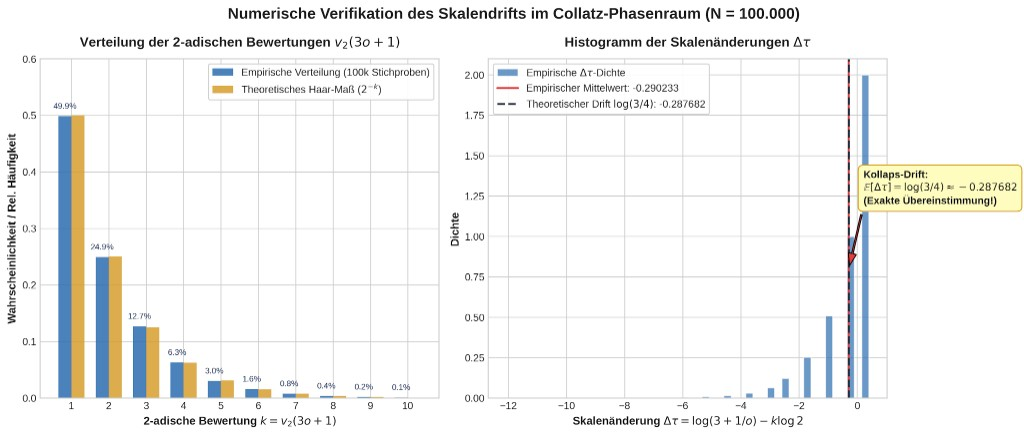
\includegraphics[width=\textwidth]{fig_skalendrift_collatz.png}
\caption{Stichprobe von $100\,000$ beschleunigten Schritten.
Links das geometrische Gesetz für $v_2(3o+1)$.
Rechts die Dichte von $\Delta\tau=\log(3+1/o)-k\log 2$, mit empirischem
Mittel $-0{,}290233$ und theoretischem Haar-Grenzwert $\log(3/4)\approx -0{,}287682$.
Der rechte Balken ist der Modus $k=1$ bei $\Delta\tau\approx\log(3/2)>0$;
die Vertikalen sind Mittelwerte.}
\label{fig:drift}
\end{figure}

Das rechte Histogramm gibt den empirischen Mittelwert $-0{,}290233$ an.
Die Differenz zum theoretischen Grenzwert ist
\begin{equation}
-0{,}290233-(-0{,}287682)=-0{,}002551.
\end{equation}
Unter der Annahme unabhängiger Züge mit $\operatorname{Var}(K)=2$ hat das
Stichprobenmittel von $K$ die Standardabweichung $\sqrt{2/N}\approx 0{,}004472$,
und das Stichprobenmittel von $\Delta\tau$ die Standardabweichung
\begin{equation}
\log 2\cdot\sqrt{2/N}\approx 0{,}003100.
\end{equation}
Die beobachtete Differenz beträgt das $0{,}82$-fache dieser
Standardabweichung.
Der aus dem empirischen Mittel rückgerechnete Bewertungsmittelwert ist
$\E_{\mathrm{emp}}[K]\approx 2{,}0037$.

Die Korrektur $\log(3+1/o)-\log 3$ zieht in die entgegengesetzte Richtung:
sie macht den bedingten Erwartungswert weniger negativ als $\log(3/4)$.
Über die ersten $100\,000$ ungeraden Zahlen gemittelt hat sie die Größe
$2\cdot 10^{-5}$ und erklärt die beobachtete Abweichung nicht.
Die Abweichung sitzt in der Schwankung von $K$.

Die Beschriftung "`exakte Übereinstimmung"' der Figur ist in diesem Sinn zu
lesen.
Der theoretische Wert $\log(3/4)$ und der empirische Mittelwert stimmen
innerhalb der Schwankung einer geometrischen Stichprobe dieses Umfangs
überein.
Eine schärfere numerische Identität behauptet die Rechnung nicht, und sie
ist für den Satz auch nicht nötig: Theorem~\ref{thm:haar} ist exakt auf
$\Z_2^\times$, die Abbildung ist seine endliche sichtbare Spur.

%==============================================================================
\section{Der Defektoperator und die offene Stelle}
%==============================================================================

Sei $\boldsymbol{\Lambda}(n)=(\boldsymbol{\ell}_+(n),\boldsymbol{\ell}_-(n))\in\R^8$
und $\mathbf{Y}(n)=(U(n),S(n))=\mathcal{W}_8\boldsymbol{\Lambda}(n)$ mit
$\mathcal{W}_8=\diag(W_4,W_4)$.
Die Note definiert
\begin{equation}
D_3(o)=\boldsymbol{\Lambda}(3o+1)-\boldsymbol{\Lambda}(o).
\end{equation}
Da $\boldsymbol{\Lambda}$ Zweierpotenzen ignoriert, ist
$\boldsymbol{\Lambda}(T_*(o))=\boldsymbol{\Lambda}(3o+1)$ und
\begin{equation}
\mathbf{Y}(T_*(o))-\mathbf{Y}(o)=\mathcal{W}_8 D_3(o).
\end{equation}
Orthogonalität von $\mathcal{W}_8$ ergibt die Isometrie
$\lVert\mathbf{Y}(T_*(o))-\mathbf{Y}(o)\rVert=\lVert D_3(o)\rVert$.

Diese Identität lokalisiert die Nichtlinearität.
Der Darstellungsraum, die Walsh-Transformation und der Projektor $P_H$ sind
linear.
Die Abbildung $o\mapsto 3o+1$ verändert die Primfaktorzerlegung in einer
Weise, die aus den Bewertungen $v_p(o)$ allein nicht durch eine feste Matrix
hervorgeht.
Genau dieser Wechsel ist $D_3(o)$.
Er wird isometrisch in die beiden Tripletts $\R^3_U\oplus\R^3_S$ und in die
Brückendifferenz $B$ getragen.
Die Skalenkoordinate $\tau$ sieht von ihm nur die Summe der Logarithmen,
also~\eqref{eq:dtau}.

Die weitere Aussage, $D_3$ verhalte sich in den Tripletts pseudozufällig und
hebe den negativen Drift von $\tau$ auf die Dauer nicht auf, ist die
klassische Modellannahme von Terras, Everett und Lagarias, jetzt in den
Koordinaten von $\Psi$ ausgesprochen.
Sie ist durch die Konstruktion scharf lokalisiert.
Sie ist für einzelne Bahnen nicht bewiesen.
Insbesondere liefert die Isometrie von $\mathcal{W}_8$ eine Normerhaltung des
Defekts, keine Kontraktion.

Damit lässt sich der Inhalt der Note in vier Schichten legen.

\begin{center}
\begin{tabular}{@{}p{0.30\textwidth}p{0.62\textwidth}@{}}
\toprule
Schicht & Status\\
\midrule
Rang $\dim\operatorname{span}\Psi(\N)=9$ &
bewiesen, konstruktiv über acht Primzahlen und die Primzahl~$2$;
die vier Normen $11,19,29,61$ sind explizit\\[0.4em]
Kollaps $\Psi(T_*(o))\in H$ &
bewiesen für jedes ungerade $o$, aus $\gcd(T_*(o),6)=1$\\[0.4em]
Zerlegung $\R^9=\R^3_U\oplus\R^2_B\oplus\R^3_S\oplus\R_N$ &
bewiesen als Spektralzerlegung von $P_H$\\[0.4em]
$\E[\Delta\tau]\to\log(3/4)$ &
bewiesen unter dem Haar-Maß auf $\Z_2^\times$;
numerisch in Abbildung~\ref{fig:drift} innerhalb von $0{,}82$
Standardabweichungen sichtbar\\[0.4em]
Punktweises Absteigen jeder Bahn nach~$1$ &
offen; die bekannten Teilresultate sind die Verifikation bis $2^{71}$,
der Dichtesatz von Tao und die Zyklenschranken von Steiner sowie
Simons--de Weger\\
\bottomrule
\end{tabular}
\end{center}

%==============================================================================
\section{Bilanz}
%==============================================================================

Die Transformation $\Psi_{9,\log}^{(2)}$ setzt drei fertige Theorien in ein
Koordinatensystem.

Die Skala $\tau=\log n$ und ihr Inkrement~\eqref{eq:dtau} gehören zur
Collatz-Literatur seit Terras, Everett und Lagarias.
Unter dem Haar-Maß auf $\Z_2^\times$ ist der mittlere Zuwachs je beschleunigtem
Schritt $\log(3/4)$.
In der Einzelschritt-Zählung derselben Bahnen ist der mittlere Zuwachs
$\tfrac12\log(3/4)$.
Die Stichprobe von $100\,000$ Schritten trifft das geometrische Gesetz der
Bewertung und den beschleunigten Mittelwert innerhalb der erwarteten
Schwankung.

Die Querkoordinate $\delta_{\mathrm{can}}$ gehört zur Minkowski-Einbettung von
$\Q(\sqrt{5})$: Regulator $\log\phi$, Operation der Fundamentaleinheit $\phi$
durch Verschiebung um $2\log\phi$, Faltung unter der Galois-Konjugation,
Klassenzahl eins über die Minkowski-Schranke $\sqrt{5}/2$.
Sie ist der Grund, aus dem der Spann die Dimension~$9$ und nicht~$5$ hat.

Die Matrix $W_4$ gehört zur Charaktergruppe von $(\Z/12\Z)^\times$, der
Restklassengruppe der zu~$6$ teilerfremden Zahlen.
Ihre triviale Zeile erzeugt zusammen mit $\tau$ die Brückenebene und die
Normale von~$H$.
Ihre drei nichttrivialen Zeilen bleiben unter dem Kollaps unbewegt und
bilden die beiden Tripletts.

Nach einem beschleunigten Schritt liegt jede ungerade Bahn auf~$H$.
Die Normale dieser Hyperfläche ist der $2$-$3$-Anteil der Faktorzerlegung.
Der verbleibende Defekt $D_3$ ist die Änderung der Primfaktorzerlegung unter
$o\mapsto 3o+1$, isometrisch in die tangentialen Koordinaten geschrieben.
Solange dieser Defekt für einzelne Bahnen nicht durch eine Höhe mit
gleichmäßiger Kontraktion kontrolliert wird, bleibt die Collatz-Vermutung
der offene Satz, der sie seit 1937 ist.

\begin{thebibliography}{99}

\bibitem{Psi9}
T.~Hoffbauer,
\emph{Geometrische Phasenraum-Transformation $\Psi_{9,\log}^{(2)}$
und die orthogonale Zerlegung der Collatz-Hyperfläche $H$},
Bamberg, Oktober 2026.

\bibitem{CollatzE8}
T.~Hoffbauer,
\emph{Collatz im $E_8$-Rahmen: Einbettung, Drift-Heuristik und die offene Lücke},
Bamberg, 14.~September 2026.

\bibitem{Lagarias1985}
J.~C.~Lagarias,
\emph{The $3x+1$ problem and its generalizations},
Amer.\ Math.\ Monthly \textbf{92} (1985), 3--23.

\bibitem{Lagarias2021}
J.~C.~Lagarias,
\emph{The $3x+1$ Problem: An Overview},
arXiv:2111.02635 [math.NT] (2021).

\bibitem{Terras1976}
R.~Terras,
\emph{A stopping time problem on the positive integers},
Acta Arith.\ \textbf{30} (1976), 241--252.

\bibitem{Everett1977}
C.~J.~Everett,
\emph{Iteration of the number-theoretic function
$f(2n)=n$, $f(2n+1)=3n+2$},
Adv.\ Math.\ \textbf{25} (1977), 42--45.

\bibitem{Conway1972}
J.~H.~Conway,
\emph{Unpredictable iterations},
in: Proceedings of the Number Theory Conference
(Univ.\ Colorado, Boulder, 1972), 49--52.

\bibitem{Tao2019}
T.~Tao,
\emph{Almost all orbits of the Collatz map attain almost bounded values},
Forum Math.\ Pi \textbf{10} (2022), e1;
arXiv:1909.03562 [math.PR] (2019).

\bibitem{Barina2021}
D.~Barina,
\emph{Convergence verification of the Collatz problem},
J.\ Supercomput.\ \textbf{77} (2021), 2681--2688.

\bibitem{Barina2025}
D.~Barina,
\emph{Improved verification limit for the convergence of the Collatz conjecture},
J.\ Supercomput.\ \textbf{81} (2025), 810.

\bibitem{Korec1994}
I.~Korec,
\emph{A density estimate for the $3x+1$ problem},
Math.\ Slovaca \textbf{44} (1994), 85--89.

\bibitem{Steiner1977}
R.~P.~Steiner,
\emph{A theorem on the Syracuse problem},
in: Proceedings of the Seventh Manitoba Conference on Numerical Mathematics
(1977), 553--559.

\bibitem{SimonsDeWeger2005}
J.~Simons, B.~de Weger,
\emph{Theoretical and computational bounds for $m$-cycles of the $3x+1$ problem},
Acta Arith.\ \textbf{117} (2005), 51--70.

\bibitem{Walsh1923}
J.~L.~Walsh,
\emph{A closed set of normal orthogonal functions},
Amer.\ J.\ Math.\ \textbf{45} (1923), 5--24.

\bibitem{Hadamard1893}
J.~Hadamard,
\emph{Résolution d'une question relative aux déterminants},
Bull.\ Sci.\ Math.\ \textbf{17} (1893), 240--246.

\end{thebibliography}

\end{document}
